\section{Syntax Highlighting, Formulas, and Questions}
\label{sec:extensions}

The previous sections covered standard Markdown and the constructs the common dialects agree on.
Lecture notes often contain three more things.
Code blocks are standard, but many Markdown viewers color them while the platform does not.
Formulas are usually written with dollar signs, but the platform only renders them in a different
notation.
Single- and multiple-choice questions, supported by H5P, have no syntax in Markdown at all.
To bridge these differences, the converter colors code during conversion and translates formula delimiters.
It also adds a syntax for questions that remains valid Markdown in other tools.

\subsection{Syntax Highlighting}
\label{sec:ex_code}

Markdown renderers commonly use a fenced code block's info string (the text after the opening backticks) to identify its language and apply appropriate syntax highlighting.
Neither Moodle nor the H5P libraries include a highlighter, and a package cannot bring one, since
\code{script} is removed by the sanitizer and JavaScript files cannot be included as content assets.
The coloring therefore has to happen during the conversion, and the colors have to be part of the
markup, i.e., applied via a tag.
The tag has to be permitted, styleable via the \code{color} property, and suitable for representing inline content,
making \code{span} the best fit (\autoref{tab:allowed}).

The converter splits every fenced code block into tokens and wraps every colored token in
\code{<span style="color:\#\ldots">}.
For this tokenization, the converter uses the lexer of RSyntaxTextArea~\cite{RSyntaxTextArea}, a Java
text component whose highlighting engine can be used without its graphical parts.
It supports more than 50 languages and 39 token types and keeps the state of multi-line comments across lines.
The converter maps the first word of a fence's info string to one of these languages, and each token
type to a color chosen for the light background of the code box.
To limit the size of the generated JSON, adjacent tokens with the same color are merged into one
span.
Identifiers, whitespace, separators, and operators, which make up the bulk of a file, receive
no span at all.
For a language without a mapping, the block remains uncolored, and one warning is issued per language
and chapter.
Some mappings are approximations: TOML is tokenized as INI and \code{.env} files as Java properties.

Three alternatives were considered.
Prism4j, a Java port of the Prism.js highlighter, supports about twenty languages but has not been
maintained since 2019.
highlight.js on the GraalVM JavaScript engine supports far more languages but requires a JavaScript
runtime in the distribution.
A custom lexer would have no dependency but would have to be written for every language.
Even so, the chosen approach has two drawbacks.
The generated \code{content.json} grows, since a colored block is several times the size of a plain
one.
The colors are also fixed, so they do not adapt to a dark mode or to the Moodle theme, since no
stylesheet can be shipped.

\subsection{Formulas}
\label{sec:ex_math}

Most Markdown editors and viewers render \code{\$x\$} as an inline formula and \code{\$\$x\$\$} as a
displayed one.
In H5P, formulas are rendered by \code{H5P.MathDisplay}, a site-wide add-on that an administrator
installs and that renders formulas in any content whose text matches its delimiters.
It recognizes \code{\textbackslash(x\textbackslash)}, \code{\textbackslash[x\textbackslash]}, and
\code{\$\$x\$\$}, but not a single dollar sign, and the delimiters cannot be configured in current
versions~\cite{H5P:MathDisplay}.
Only \code{\$\$x\$\$} is therefore understood by both sides, but the most common Markdown notation for
inline formulas would be displayed as literal dollar signs.

The converter recognizes both dollar notations and only rewrites the one that needs it.
\code{\$x\$} becomes \code{\textbackslash(x\textbackslash)}, while \code{\$\$x\$\$} is kept as it is,
so that it also reads correctly on a site without the add-on.
On the H5P side, nothing else is needed, since the add-on finds the delimiters in the rendered page.
On the Markdown side, a custom extension to commonmark was implemented.
Without it, commonmark would interpret the asterisks in \code{\$a*b*c\$} as emphasis.
The extension changes single-dollar delimiters to \code{\textbackslash(} and \code{\textbackslash)} and prevents the formula's contents from being interpreted as Markdown.
Since \code{\$5} and \code{\$PATH} are common in documentation, though, single-dollar formulas need a rule.
The converter uses that of Pandoc: no whitespace directly inside either delimiter and no digit right
after the closing one.
As a consequence, \code{\$ x \$} is not recognized as a formula.

The backslash notations are not treated as formulas in the source.
Markdown editors generally do not render \code{\textbackslash(x\textbackslash)} as math, so an author who wrote it
meant an escaped parenthesis, and their preview shows \code{(x)}.
commonmark's backslash escape already turns \code{\textbackslash(} into \code{(}, so the add-on finds
no delimiter.
Even with these delimiter changes, two limitations remain.
Formulas are only rendered if the add-on is installed, which the package cannot check; otherwise the
reader sees \code{\textbackslash(E = mc\textasciicircum{}2\textbackslash)}.
Furthermore, a vertical bar inside a formula still splits a table cell, since the table extension
determines the cell boundaries before inline parsing.

\subsection{Interactive Questions}
\label{sec:ex_quiz}

Markdown has no syntax for questions, so one has to be defined.
The main requirement is that the file still works in every other tool the author uses, such
as Obsidian, GitHub's viewer, or an editor's preview.
A format that only this converter can read would no longer be Markdown.
The syntax therefore has to render as something sensible in other tools, and its content has to be
protected from other parsers, since it is not prose.

A fenced code block meets both requirements.
It is part of CommonMark and thus supported by every tool, its content is taken literally, and its
info string is free text without a predefined meaning.
In other tools, the author sees a small monospaced box with the question and its answers.
\autoref{lst:quiz} shows the syntax.
The info string names the question type (\code{singlechoice} to create an \code{H5P.SingleChoiceSet} block and \code{multiplechoice} for an \code{H5P.MultiChoice} block), the first line is the question, and every further line is an
answer.
A leading asterisk marks a correct answer.

\par\medskip
\noindent\begin{minipage}{\linewidth}
\begin{lstlisting}[morecomment={[l][\color{blue!60!black}]{```}},caption={[Example questions as fenced code blocks]A single-choice and a multiple-choice question as fenced code blocks.
The info string selects the type, the first line is the question, and a leading asterisk marks a
correct answer.},label={lst:quiz}]
```singlechoice
What is the capital of Austria?
Salzburg
*Vienna
Linz
```

```multiplechoice
Which of these are H5P content types?
*Interactive Book
Markdown
*Course Presentation
\*.h5p (this answer starts with a literal asterisk)
```
\end{lstlisting}
\end{minipage}

The info string could also support future extensions, such as flashcards and fill-in-the-blank questions.

\begin{figure}[H]
	\centering
	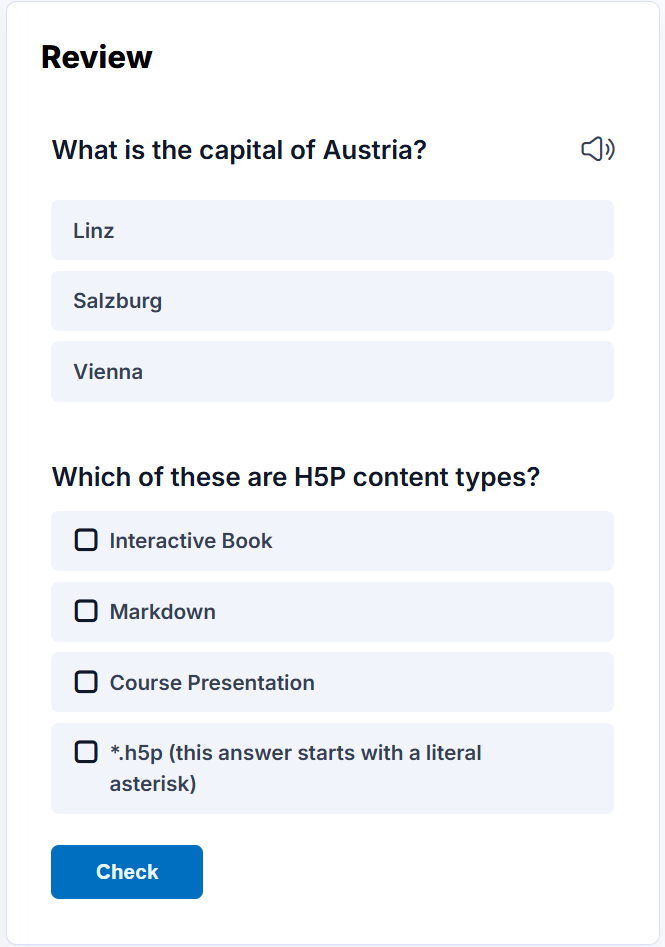
\includegraphics[width=0.55\columnwidth]{figures/screenshots/quiz}
	\caption[The example questions in Moodle]{\label{fig:quiz}The questions of \autoref{lst:quiz} in Moodle.}
\end{figure}

\autoref{fig:quiz} shows both questions of \autoref{lst:quiz} as the reader sees them.

A block that cannot become a question because it is empty, has no answers, only one answer, or
no correct answer becomes an ordinary code block with a warning naming the problem.
